\documentclass{acm_proc_article-sp}

\usepackage{url, fancyvrb, framed, multirow, tabularx, graphicx, epstopdf, enumerate}

\begin{document}

\title{NDN Repo: An NDN Persistent Storage Model}

\numberofauthors{3}

\author{
% 1st. author
\alignauthor
Shuo Chen\\
	\affaddr{Research Institute of Information}\\
	\affaddr{Tsinghua University}\\
	\affaddr{Beijing, China}\\
	\email{chenatu2006@gmail.com}
}
\maketitle

\begin{abstract}
NDN repository (repo for short) is persistent storage model of Named Data Networking, compared with NDN Content Store. NDN makes in-network storage possible because of naming and signature of network layer data packet. NDN repo is not a built-in part of NDN, but built upon application layer without tweaking NDN protocol. A specification of NDN repo is designed to standardize repo operation interfaces. Retrieval, insertion and deletion of data objects are supported in this specification and basic semantics of repo commands is defined.

In this paper, details of NDN repo specification are demonstrated and an initial implementation based on ndn-cxx library and sqlite3 is presented. (Something about the evaluation results)

\end{abstract}

\section{Introduction}
Named Data Networking (NDN) \cite{zhang2010named} is a data-oriented network architecture which replaces IP with names of the data packets as narrow waist of networking. The essential evolution of NDN is the change of network behavior from delivering data to a certain destination to fetching data with a given name. \cite{zhang2010named} Because of this change, \emph{interest} and \emph{data object} are two kinds of network packet for fetching and returning data of given name. \emph{Interest} is the request of network packet containing prefix of name and other constraints. Besides the content of data packet, data packet also contains the full name and signature of data.

Naming and signature of data makes in-network storage possible because of the following reasons. Network packet in named by source and destination host addresses in IP network, while name of NDN packet is irrelevant with physical endpoints. Any host in NDN network carrying data of given name can response to the \emph{interest}, but hosts besides source and destination cannot retrieve in-network IP packet. Another concern is the privacy of in-network data. Signature in data packet is to resolve authentication and confidentiality of data. \emph{Content Store (CS)} is cache of data packet in NDN router model and it is within network layer. NDN repository (Repo for short) is persistent NDN storage model. It is an application conforming to NDN protocol and can be used as storage functional components by other NDN applications such as video streaming and CDN like applications.

\emph{Ccnr} proposed by Project CCNx, which also serves as persistent storage of data packets just provides read and write access of content object. It does not support deletion of data packet and does not provide any validation and access control. Compared to CCNx Repository Protocol, a more functional specification is proposed to provide remote operations of repo in this paper. Three basic functions including retrieving, inserting and deleting data packets are supported in addition with check of insertion and deletion progress. Validation of command interest is supported for authentication.

An implementation of NDN repo protocol \emph{repo-ng} (repo of new generation) is also demonstrated in this paper. The NDN repo protocol is implemented in repo-ng. It is developed with ndn-cxx and uses sqlite3 for storage of data packets and in-memory index for high speed query.

The rest of the paper is organized as follows: section 2 demonstrates the details of NDN repo protocol, section 3 describes the implementations of repo-ng, section 4 evaluated the performance of repo-ng and section 5 concludes the paper and discusses the future work.

\section{NDN REPO PROTOCOL DESIGN}
\subsection{Overview}

A repo preserves content and responds to interests requesting content that it holds. A Repo can exist in any node, and is recommended for applications to preserve the data. The NDN repo protocol is a specification of repo operations including reading, insertion and deletion of emph{content objects} in repo. Compared to \emph{ccnr} proposed in Project CCNx, insertion and deletion are supported in this protocol by \emph{signed command interest}. The repo protocol does not stipulated on certain trust model, but practical application could define its trust model and policy of access control.

Retrieving data from repo is just like common ways of retrieving data from NDN network. \emph{Repo command} based on singed interest is used to support insertion and deletion function. Validation and access control can be designed based on signed components. A new repo semantics different from NDN semantics is defined for \emph{repo command}.

\subsection{Retrieving Data}

  Repo registers prefixes of data objects it holds into NDN forwarding daemon (NFD) and the repo will respond the data with such prefixes. A standard interest is used to fetch content from the repo. The repo will start to search the data packet when the name of the interest matches the prefix it registered in NFD. If the data packet in repo matches the interest, it will respond with this \emph{data packet}. When the interest is not matched, it will not respond. The following figures shows the process of retrieving data.

\begin{figure}
\centering
\includegraphics{Drawing1.eps}
\caption{Retrieving data that matches in repo}
\end{figure}

\begin{figure}
\centering
\includegraphics{Drawing2.eps}
\caption{Retrieving data that does not match in repo}
\end{figure}

\subsection{Repo Command and Repo Command Response}
Four types of commands are supported in repo protocol: insertion, deletion, insertion status check and deletion status check. Repo command is a based on signed interest \cite{signed-interest}. Repo command response is a specific type of NDN data packet conforming to the following specification.

\subsubsection{Background}
NDN packets \cite{ndn-packet} are encoded in a Type-Length-Value (TLV) format. One TLV block can be nested with servral sub TLV bocks and the length of each TLV block is variable. The type of block is defined in the first few octets and the length of block is set subsequently. Wired format of name is just a sub TLV block of interest and all the components of name are nested in the name block.

Repo command interests are based on signed interests. Signed interests is used for authentication. The signed interests not only contain cryptographic signature, but also ensure uniqueness of each command. The following name is a typical structure of name of singed interest. For /signed/interest/name name, Command Interest will be defined as:

\begin{figure*}[htbp]
\centering
\begin{framed}
\begin{BVerbatim}
 /signed/interest/name/<timestamp>/<random-value>/<SignatureInfo>/<SignatureValue>
                       \                                                         /
                        -------------------------  ------------------------------
                                                \/
                              Additional components of Command Interest
\end{BVerbatim}
\end{framed}
\end{figure*}

n denotes the count of components of name. The n-3th is the timestamp of command to protect replay attack. The n-2th is random value that guarantee the uniqueness of the command. The n and n-1th components are signature and signature info of the interest for validation.

\subsubsection{Repo Command}
Repo commands are encoded in the form of signed interest. The semantics of repo command interest is as follows.

The name semantics is defined to have following components:

\begin{itemize}
\item <repo prefix> refers to specific prefix repo is listening
\item <command verb> refers to the name of command
\item <RepoCommandParameter> refers to parameters of repo command
\end{itemize}

The following components are components of singed interest for access control:
\begin{itemize}
\item <timestamp>
\item <random-value>
\item <SignatureInfo>
\item <SignatureValue>
\end{itemize}

For prefix of repo /ucla/cs/repo/, the command will be defined as this:

\begin{figure*}
\begin{framed}
\begin{BVerbatim}
/ucla/cs/repo/<command verb>/<RepoCommandParameter>/<timestamp>/<random-value>/<SignatureInfo>
/<SignatureValue>
\end{BVerbatim}
\end{framed}
\end{figure*}

The RepoCommandParatmeter component is also nested with sub TLV component. It defines as follows:

\begin{figure*}
\begin{framed}
\begin{BVerbatim}
RepoCommandParameter ::= REPOCOMMANDPARAMETER-TYPE TLV-LENGTH
                           Name?
                           Selectors?
                           StartBlockId?
                           EndBlockId?
                           ProcessId?

Name                  ::= NAME-TYPE TLV-LENGTH NameComponent*
NameComponent         ::= NAME-COMPONENT-TYPE TLV-LENGTH BYTE+

Selectors             ::= SELECTORS-TYPE TLV-LENGTH
                           MinSuffixComponents?
                           MaxSuffixComponents?
                           PublisherPublicKeyLocator?
                           Exclude?
                           ChildSelector?

MinSuffixComponents   ::= MIN-SUFFIX-COMPONENTS-TYPE TLV-LENGTH
                           nonNegativeInteger

MaxSuffixComponents   ::= MAX-SUFFIX-COMPONENTS-TYPE TLV-LENGTH
                           nonNegativeInteger

PublisherPublicKeyLocator ::= KeyLocator

Exclude               ::= EXCLUDE-TYPE TLV-LENGTH Any? (NameComponent (Any)?)+
Any                   ::= ANY-TYPE TLV-LENGTH(=0)

ChildSelector         ::= CHILD-SELECTOR-TYPE TLV-LENGTH
                           nonNegativeInteger

StartBlockId          ::= STARTBLOCKID-TYPE TLV-LENGTH
                           nonNegativeInteger

EndBlockId            ::= ENDBLOCKID-TYPE TLV-LENGTH
                           nonNegativeInteger

ProcessId             ::= PROCESSID-TYPE TLV-LENGTH
                           nonNegativeInteger
\end{BVerbatim}
\end{framed}
\end{figure*}

Name adopts the same TLV structure of name of interest and data packet. This name denotes the name of possessed data. Selectors adopt the same TLV structure of selector\cite{selector}. However, only parts of selectors including MinSuffixComponents, MaxSuffixComponents, PublisherPublicKeyLocator, Exclude, and ChildSelector are used in repo command parameter. The meaning of selectors is not the same in different operations which will be discussed in the following sections. StartBlockId and EndBlockId denotes the beginning and end of segment number to support segmented insertion and deletion. ProcessId is a random number generated to identify operation process. It is used for insertion and deletion status check.

\subsubsection{Repo Command Response}
Repo command response is the response data packet of repo command interest. The response contains statuscode to indicate the status of command process and other information. A TLV-encoded block called RepoCommandResponse is encoded in content block of the data packet. It defines as follows:

\begin{figure*}
\begin{framed}
\begin{BVerbatim}
RepoCommandResponse   ::= INSERTSTATUS-TYPE TLV-LENGTH
                           ProcessId?
                           StatusCode
                           StartBlockId?
                           EndBlockId?
                           InsertNum?
                           DeleteNum?

ProcessId             ::= PROCESSID-TYPE TLV-LENGTH
                            nonNegativeInteger

StatusCode            ::= STATUSCODE-TYPE TLV-LENGTH
                            nonNegativeInteger

StartBlockId          ::= STARTBLOCKID-TYPE TLV-LENGTH
                            nonNegativeInteger

EndBlockId            ::= ENDBLOCKID-TYPE TLV-LENGTH
                            nonNegativeInteger

InsertNum             ::= INSERTNUM-TYPE TLV-LENGTH
                            nonNegativeInteger

DeleteNum             ::= DELETENUM-TYPE TLV-LENGTH
                            nonNegativeInteger

\end{BVerbatim}
\end{framed}
\end{figure*}

The TLV structure and meaning of Name, ProcessId, StartBlockId, and EndBlockId are just like those of RepoCommandParameter. InsertNum is the count of data inserted. DeleteNum is the count of data erased. Statuscode is the number indicating the status of command. The detailed definition will be introduced in the following sections.

\subsubsection{Repo TLV Type Encoding Number}

In TLV encoding, first several bits defines the type of block. Table 1 shows these codes definition

\begin{table}[!hbp]
\centering

\begin{tabular}{l l}

\hline
type & number \\
\hline
RepoCommandParameter & 201 \\
StartBlockId & 204 \\
EndBlockId & 205 \\
ProcessId & 206 \\
RepoCommandResponse & 207\\
StatusCode & 208 \\
InsertNum & 209 \\
DeleteNum & 210 \\
\hline

\end{tabular}
\caption{Repo TLV Type Encoding Number}
\end{table}



\subsection{Authentication and Authorization}
The trust model and access control of repo depends on specific implementation. The protocol does not limit type of trust model. The implementation of repo can either adopt policy based or reputation based trust model for validation the repo command interest. The protocol only requests signature and timestamp for repo command interest. Access control is also defined by specific implementation. Public key in signature is a good identifier for access control list.

\subsection{Inserting Data and Insertion Status Check}

Repo insertion command requests that the repo retrieves and stores content from requester. Validation of commands is defined by specific implementation. When the intereste is validated and name of the data is not existed in the repo. The repo will response with a data object containing OK status and start to send the interest to fetch the data to insert.

Segmented data insertion is also supported in the insertion protocol. Segmentation information is defined in RepoCommandParameter.

Command of insertion status check is supported. Once the check command was sent, repo will return response about the first and the last of id of segmented data and how many blocks have been inserted. If EndBlockId Missing Timeout is allowed, this check command can also reset the timer to zero.

\subsubsection{2.5.1	Structure of Repo Insertion Command and Insertion Status Check Command}
The name semantics follows the format of the repo command. The ``<command verb>'' are defined as ``insert'' and ``insert check''. For example, for <repo prefix> as /ucla/cs/repo, the following are an examples of insertion and insertion check command:

\begin{figure*}
\begin{framed}
\begin{BVerbatim}

/ucla/cs/repo/insert/<RepoCommandParameter>/<timestamp>/<random-value>/<SignatureInfo>/<SignatureValue>

\end{BVerbatim}
\end{framed}
\end{figure*}

\begin{figure*}
\begin{framed}
\begin{BVerbatim}

/ucla/cs/repo/insert check/<RepoCommandParameter>/<timestamp>/<random-value>/<SignatureInfo>/<SignatureValue>

\end{BVerbatim}
\end{framed}
\end{figure*}


\subsubsection{RepoCommandParameter of Insertion Command}
RepoCommandParameter of insertion command follows TLV structure of RepoCommandParameter of repo command, but adopts only parts of sub TLV-block including, Name, Selector, StartBlockId, EndBlockId. The name section is a must section in this scenario.

\begin{itemize}
\item <Name> indicates the prefix of name of data that will be inserted into repo.
\item <Selector> indicates the selectors of interests for repo to fetch data.
\item <StartBlockId> indicates the first segment ID of segmented data to be inserted.
\item <EndBlockId> indicates the last segment ID of segmented data to be inserted.
\end{itemize}

\subsubsection{RepoCommandParameter of Insertion Check Command}
RepoCommandParameter of insertion check command follows TLV structure of RepoCommandParameter of repo command, but only and must adopt ProcessId.

\begin{itemize}
\item <ProcessId> is retrieved from the RepoCommandResponse of Insertion Command and it indicates the identity of the insertion progress.
\end{itemize}

\subsubsection{RepoCommandResponse of Insertion Command}
RepoCommandResponse of insertion command follows TLV structure of RepoCommandResponse. Once the interest arrives, repo will validate the repo command and check the authorization of the command. Then Repo will return the response according to the result of command validation. RepoCommandResponse of insertion adopts ProcessId, StatusCode, StartBlockId, EndBlockId, and InsertNum sections. StatusCode is the must section.

\begin{itemize}
\item <ProcessId> is generated when the interest is validated and authorized.
\item <StatusCode> indicates status of insertion status.
\item <StartBlockId> indicates the first segment ID of segmented data to be inserted.
\item <EndBlockId> indicates the last segment ID of segmented data to be inserted.
\item <InsertNum> indicates how many content objects have been inserted.
\end{itemize}

\subsubsection{RepoCommandResponse of Insertion Status Check Command}
RepoCommandResponse of insertion status check command follows TLV structure of RepoCommandResponse. Once the interest arrives, repo will validate the command interest and check the authorization of the command. Then Repo will check the insertion status according to ProcessId. RepoCommandResponse of insertion check adopts ProcessId, StatusCode, StartBlockId, EndBlockId, and InsertNum sections. StatusCode and ProcessId are the must sections.

\begin{itemize}
\item <ProcessId> is the same with that of insertion response.
\item <StatusCode> indicates status of insertion progress.
\item <StartBlockId> indicates the first segment ID of segmented data to be inserted.
\item <EndBlockId> indicates the last segment ID of segmented data to be inserted.
\item <InsertNum> indicates how many content objects have been inserted.
\end{itemize}

The following table shows the definition of StatusCode.

\begin{table}[!hbp]
\centering

\begin{tabular}{l l}

\hline
StatusCode & Description \\
\hline
100 & The command is OK. can start to fetch the data \\
200 & All the data has been inserted \\
300 & This insertion is in progress \\
401 & This insertion command or insertion check command is invalidated \\
402 & Selectors and BlockId both present\\
403 & Malformed Command \\
404 & No such this insertion is in progress \\
\hline

\end{tabular}
\caption{StatusCode of Insertion}
\end{table}

\subsubsection{Types of Insertion}
There are 3 types of supported insertion: name, selector and segment.

Name insertion means repo expresses interest just containing name of inserted data. Selector, StartBlockId and EndBlockId are all not set, except Name of RepoCommandParameter.

Selector insertion means inserting one content object conforming to Name as prefix and Selector. StartBlockId and EndBlockId will not be set. Name and Selector will be set.

Segment insertion means inserting multiple segmented content objects into the repo. Selector will not be set. At least one of StartBlockId and EndBlockId is set.

\subsubsection{EndBlockId Missing Timeout}
If StartBlockId presents but EndBlockId is missing, and returned data packets do not contain FinalBlockId, the repo will continuously fetch the data. An EndBlockId Missing Timeout is set to prevent this occasion. The repo will start a timer when StartBlockId presents but EndBlockId and FinalBlockId are missing. When timeout happens, repo will stop fetching data to store and end insert process. If an insert check command arrives during this insert process, the time of timer is set to 0. If data packet containing FinalBlockId arrives, this timeout timer will be dismissed.

\subsubsection{Insertion Protocol Process}

Progress of Inserting Data:

\begin{enumerate}[step 1]

\item Dtart to authorize the command; If authorization does not fail immediately, go to step 3

\item Send a negative response indicating authorization failure, and abort these steps, insert process ends (StatusCode: 401)

\item If both StartBlockId and EndBlockId are missing, go to step 7

\item If either StartBlockId or EndBlockId is present, and one of supported selectors is present. Send negative response back and abort steps, insert process ends (StatusCode: 402)

\item If both StartBlockId and EndBlockId are present, and StartBlockId is less than or equal to EndBlockId, go to step 7

\item Send a negative response indicating malformed command, and abort these steps, insert process ends (StatusCode: 403)

\item Wait for authorization completion

\item If authorization fails, go to step 2 (StatusCode: 401)

\item Send a positive response indicating insert is in progress (StatusCode: 200)

\item If either StartBlockId or EndBlockId is present, go to step 16

\item Start to retrieve Name with selectors in insert command

\item Wait for retrieval completion

\item If retrieval fails, go to step 27

\item Store retrieved Data packet

\item Abort these steps, insert process ends

\item If StartBlockId is missing, set StartBlockId 0. If EndBlockId is missing, EndBlockId will be missing unless get FinalBlockId in coming data packets, start EndBlockId Missing Timeout timer.

\item Append StartBlockId to Name

\item Start to retrieve Name

\item Wait for retrieval completion

\item If retrieval fails, go to step 26

\item Store retrieved Data packet

\item If retrieved Data packet contains FinalBlockId, and FinalBlockId is less than EndBlockId or EndBlockId is missing, let EndBlockId be FinalBlockId

\item If the last component of Name is greater than or equal to EndBlockId, abort these steps, insert process ends

\item Increment the last component of Name

\item Go to step 17

\item Retrieve data with this data another 2 times. If these 2 retrieval both fails, abort these steps. If success, go to step 21

\item Retrieve data with this data another 2 times. If these 2 retrieval both fails, abort these steps. If success, go to step 14
\end{enumerate}

If EndBlockId Missing Timeout timer starts, repo will monitor this timer during step 17~27. If this timeout occurs, abort insertion command process immediately.

Implementation MAY pipeline the Interests.

Progress of Insertion Check:

Implementation MAY publish a notification of status regarding insert progress. The process of insertion check is as follows:

\begin{enumerate}[step 1]

\item start to authorize the insert status command, if fails go to 2, if success, go to 3

\item send a negative response indicating authorization failure, and abort these steps (StatusCode: 401)

\item start to check the progress of the insert with the data name in the command. If no such progress is found, go to 4. or go to 5.

\item response status with status code, abort check process. (StatusCode: 404)

\item check the status of insertion. return the status of insertion progress. If a EndBlockId Missing Timeout timer is running, set this timer to 0. About check process. (StatusCode: 300)

\end{enumerate}

The figure 3 below shows the simple process of insertion.

\begin{figure*}
\centering
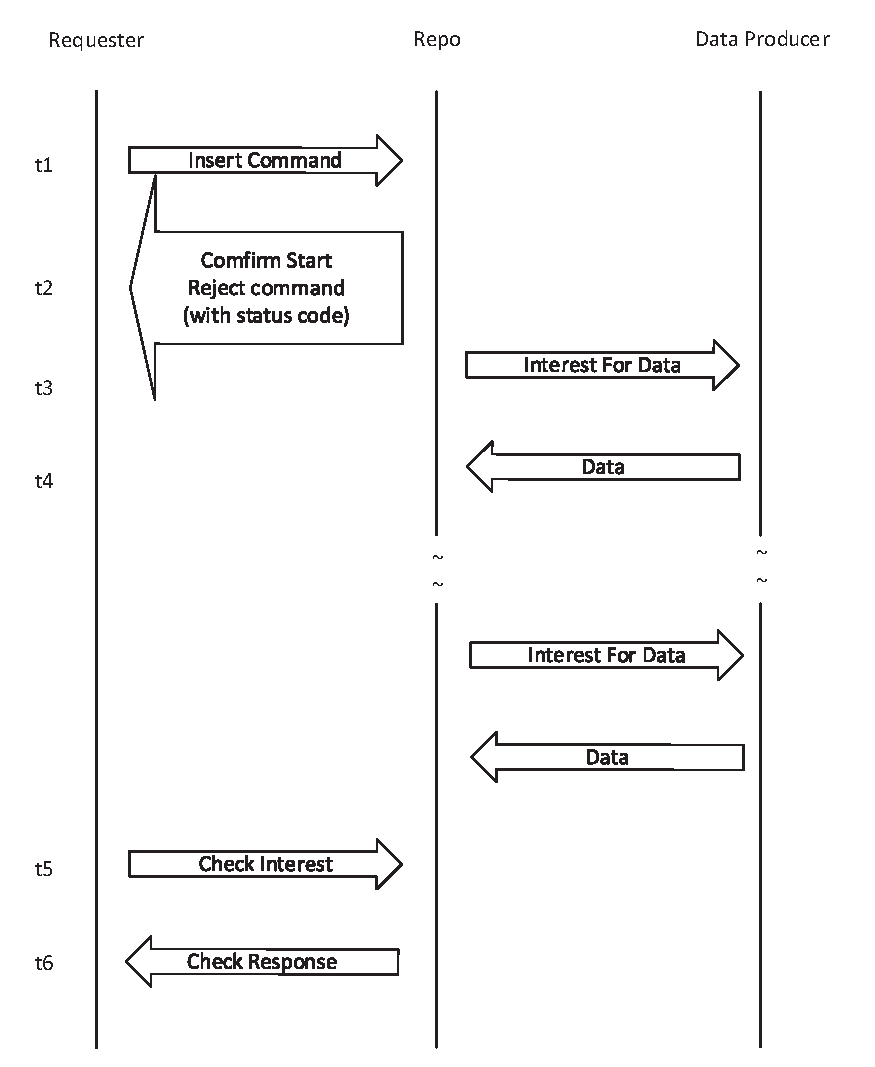
\includegraphics{Drawing3.eps}
\caption{Insertion and Insertion Status Check Progress}
\end{figure*}

\subsection{Deleting Data and Deletion Status Check}
Deletion of one content object or multiple content objects under certain prefix are both supported. Selectors can be used in deletion but have different semantics with those of insertion.

\subsubsection{Structure of Repo Deletion and Deletion Status Check Command}
The name semantics follows the format of the repo command. The ``<command verb>'' are defined as ``delete'' and ``delete check''. For example, for <repo prefix> as /ucla/cs/repo, the following are an examples of deletion and deletion check command:


\begin{figure*}
\begin{framed}
\begin{BVerbatim}

/ucla/cs/repo/delete/<RepoCommandParameter>/<timestamp>/<random-value>/<SignatureInfo>/<SignatureValue>

\end{BVerbatim}
\end{framed}
\end{figure*}

\begin{figure*}
\begin{framed}
\begin{BVerbatim}

/ucla/cs/repo/delete check/<RepoCommandParameter>/<timestamp>/<random-value>/<SignatureInfo>/<SignatureValue>

\end{BVerbatim}
\end{framed}
\end{figure*}

\subsubsection{RepoCommandParameter of Deletion Command}
RepoCommandParameter of deletion command follows TLV structure of RepoCommandParameter of repo command, and adopts all the sub-sections. The Name and ProcessId sections are the must sections in this scenario.

\begin{itemize}
\item <ProcessId> is generated by the deletion requester and it indicates the identity of the deletion progress.
\item <Name> indicates the prefix of name of data that will be deleted from repo.
\item <Selector> indicates the selectors of interests for repo to deleting data.
\item <StartBlockId> indicates the first segment ID of segmented data to be deleted.
\item <EndBlockId> indicates the last segment ID of segmented data to be deleted.
\end{itemize}

\subsubsection{RepoCommandParameter of Deletion Status Check Command}
RepoCommandParameter of deletion check command follows TLV structure of RepoCommandParameter of repo command, but only and must adopt ProcessId.

\begin{itemize}
\item <ProcessId> is that of deletion command to indicate the specific deletion progress.
\end{itemize}


\subsubsection{RepoCommandResponse of Deletion Command}
RepoCommandResponse of deletion command follows TLV structure of that of repo. Once the interest arrives, repo will validate the command interest and check the authorization of the command. Then Repo will start deletion prgress. When the deletion is finished, repo will return the response. RepoCommandResponse of deletion adopts ProcessId, StatusCode, StartBlockId, EndBlockId, and DeleteNum sections. StatusCode is the must section.

\begin{itemize}
\item <ProcessId> is generated by the deletion command interest;
\item <StatusCode> indicates status of deletion.
\item <StartBlockId> indicates the first segment ID of segmented data to be deleted.
\item <EndBlockId> indicates the last segment ID of segmented data to be deleted.
\item <DeleteNum> indicates how many content objects have been deleted.
\end{itemize}

\subsubsection{RepoCommandResponse of Deletion Status Check Command}
RepoCommandResponse of deletion check command follows TLV structure of RepoCommandResponse of repo. Once the interest arrives, repo will validate the command interest and check the authorization of the command. Then Repo will check the deletion status according to ProcessId. RepoCommandResponse of deletion check adopts ProcessId, StatusCode, StartBlockId, EndBlockId, and DeleteNum sections. StatusCode and ProcessId are the must sections.

\begin{itemize}
\item <ProcessId> is the same with that of deletion command.
\item <StatusCode> indicates status of deletion.
\item <StartBlockId> indicates the first segment ID of segmented data to be deleted.
\item <EndBlockId> indicates the last segment ID of segmented data to be deleted.
\item <DeleteNum> indicates how many content objects have been deleted.
\end{itemize}

The following table shows the definition of StatusCode.

\begin{table}[!hbp]
\centering

\begin{tabular}{l l}

\hline
StatusCode & Description \\
\hline
200 & All the data has been deleted \\
300 & This deletion is in progress \\
401 & This deletion or deletion check command is invalidated \\
402 & Selectors and BlockId both present\\
403 & Malformed Command \\
404 & No such this deletion  is in progress \\
\hline

\end{tabular}
\caption{StatusCode of Deletion}
\end{table}

\subsubsection{Types of Deletion}
There are 3 types of supported deletion: name, selector and segment.

Name deletion means deleting all the content objects with Name as their prefix. Selector, StartBlockId and EndBlockId are all not set, except Name of RepoCommandParameter.

Selector deletion means deleting any content object conforming to Name as prefix and Selector. StartBlockId and EndBlockId will not be set. Name and Selector will be set.

Semantics of selectors in this case is different. In this case, the selector will match all the content objects conforming to the selector conditions not just one content object.

Segment deletion means deleting multiple segmented content objects from the repo. Selector will not be set. At least one of StartBlockId and EndBlockId is set.


\subsubsection{Deletion Protocol Process}

Progress of Deleting Data:

\begin{enumerate}[step 1]

\item Start to authorize the command; If authorization does not fail, go to step 3

\item Send a negative response indicating authorization failure, and abort these steps, end deletion process. (StatusCode: 401)

\item Check whether a deletion process of same RepoCommandParameter exists, waiting for deletion process ends.

\item If selectors and one of StartBlockId and EndBlockId presents, send a negative response and abort these steps, end deletion process. (StatusCode: 402)

\item If selectors present, go to step 8

\item Check whether StartBlockId or EndBlockId presents. If both presents but StartBlockId is larger than EndBlockId, return negative response and end deletion process. (StatusCode: 403) Or go to step 9

\item If StartBlockId, EndBlockId and selectors are all missing, go to step 10

\item Delete all the data that conforms to the name and selectors, go to step 11

\item Delete all the data packets of segment id between StartBlockId and EndBlockId. If StartBlockId is missing, StartBlockId is set to be 0. If EndBlockId is missing, EndBlockId is set to be the largest segment id that repo holds. go to step 11

\item Delete data with prefix of Name. Go to step 11

\item If lifetime of interest does not expire, return status response of positive StatusCode. If lifetime of interest has expired, wait for interest the same RepoCommandParameter and return this status response. End Deletion process. (StatusCode: 200)

\end{enumerate}

Requester will set deletion command with big lifetime. The repo will also hold the status of deletion progress for certain duration after deletion done. If lifetime expires, client will re-express the command to get the response.

Implementation MAY publish a notification of status regarding delete progress. The process of status check is as follows:

\begin{enumerate}[step 1]

\item Start to authorize the delete status command

\item Send a negative response indicating authorization failure, and abort these steps (StatusCode: 401)

\item Start to check the progress of the delete with the data name in the command. If no such progress is found, go to 4. or go to 5.

\item Response status with status code of 404 (StatusCode: 404)

\item Check the status of delete. Return the status data content (StatusCode: 300)

\end{enumerate}

\begin{figure}
\centering
\includegraphics{Drawing4.eps}
\caption{Deletion and Deletion Status Check progress}
\end{figure}


\section{REPO-NG DESIGN}
Repo-ng (NDN repo of new generation) is an implementation of NDN persistent in-network storage conforming to NDN Repo protocol. It uses ndn-cxx as NDN client library and database Sqlite3 as underlying data storage.

\subsection{Supported Feature}

Besides supporting repo protocol, repo-ng has some tools to manipulate repo and some other features for upper application.
\begin{enumerate}
\item Get, put and delete file: tools to get, put and delete (to do) a file from repo
\item Sync: use ChronoSync \cite{zhu2013let} to synchronize data objects among different repos
\end{enumerate}

\subsection{Software Structure}

Major Modules:
\begin{itemize}
\item Storage: basic interfaces to handle storage related operations including reading, insertion, update and deletion. It also operates on NDN packets according to selectors bound with interests. This module locates in src/storage directory. The storage of repo-ng consists of index and database storage in current design which will be demonstrated more specifically in next section.
\item Handle: Handle module can handle interests or commands of different functions separately. Reading is supported in read-handle, insertion and insertion status check in write-handle and deletion and deletion status check in delete-handle. This module locates in src/handle directory.
\item Helpers: repo command parameter, response and repo TLV formats are defined in this module.
\item Server: The process of starting a repo is defined  including reading configuration file, initiating database, connection to NFD and registration of prefixes.
\item Test: unit-test and integrated tests are both supported
\item Tool: command line tools to use repo such as tools to fetch a file from, to dump a file into the repo and so on.
\end{itemize}

\subsection{Repo Storage Design}
The design of data packet storage of repo-ng consists of index and storage components. Index is sorted associative container for Name stored in memory and storage is consistent storage for read, write and delete of data packet.

Underlying storage offers structured API for retrieval, adding and removal of data packets. Sqlite3 is chosen to be the underlying storage for its well cross-platform, self-contained, serverless, and zero-configuration properties. The structure of a set of data packet is (Id, Data packet). The Id is the unique integer representing the data packet.

Index offers fast query of interest in memory. When an interest comes to repo, repo will query the index with the name and selector to select the id of data packet which is consistent with that of underlying storage. The structure of one entry of index is (Id, Name, KeyLocatorHash). Name is the name of data packet. KeyLocatorHash is the hash of key locator of data packet.

In current repo-ng design, the data structure of repo-index is skip list. \cite{pugh1990skip} Although skip list, Btree and other balanced tree all have O(n) query and insertion complexity, skip list has very low inherent constant-factor overheads. Besides, operations of skiplist are much easier to implement.


\subsection{Supported Repo Protocol Features}
Most parts of the protocol are supported in repo-ng. The following features are not supported in current version.

\begin{itemize}

\item For deletion command, if EndBlockId is null in RepoCommandParameter, repo just returns RepoCommandResponse with StatusCode 403 (Malformed Command).

\item Command for checking deletion Status

\end{itemize}

\subsection{Tust Model and Access Control}

\subsubsection{Tust Model}

Command Interest and Data Packet can both be validated by repo-ng. Whether or not validating is an option that can be configured. However, validation of command interest is highly recommended. In repo-ng implementation, ``validator-config'' which is part of NDN basic library ``ndn-cxx'' is used as validator. The configuration file follows the format of validconf. \cite{validconf}

\subsubsection{Access Control}

\subsection{Congestion Control}
In process of insertion, after repo receiving the insertion command for segmented data, it will send multiple interests for data packets. If these interests are sent in a burst, the round trip time will be large for some interests and it is difficult to set interest lifetime. So congestion control is necessary.

A basic credit based congestion control is implemented for insertion command. There is credit number to count the waiting interest request. Once an interest is sent, the credit minus one and if an interest is satisfied by one data. If credit is equal or less than 0, the repo stops sending interests. The original credit number could be adjusted according to the count of interest on the wire.

In addition, if an interest is timeout. The same interest could be retransmitted for certain times that can be configured. The retransmitted interest will not subtract the credit.

The flow chart of this congestion control is as follows:

\begin{figure*}
\centering
\includegraphics{Drawing5.eps}
\caption{Process of Congestion Control}
\end{figure*}

\section{EVALUTATION OF REPO-NG}

In this section, the performance of repo-ng including is evaluated. The speed of data fetching, insertion and deletion of data packets are measured. In addition, comparison between repo-ng over NFD platform and ccnr over ccnd platform are conducted.

Tests are conducted on different hardware platforms:
\begin{itemize}
\item Macbook Pro with 2.9 GHz Intel Core i7 processor, 8GB memory, 500GB hard drive with 7200r/min, Ethernet Card brandwidth.
\item Raspberry Pi:
\end{itemize}

Software platform:
For repo-ng, it is developed by ndn-cxx \cite{ndn-cxx} which is NDN C++ library with eXperimental eXtensions. The forwarding deamon of repo-ng is NFD. \cite{NFD} Ccnr uses ccnd \cite{ccnd} as forwarding deamon. All the software runs on Ubuntu 13.10.

\subsection{Local Access}

Repo-ng and ccnr both supports retrieving and inserting data packets, but repo-ng also supports deleting data packets from repo. In this section, all the operations are tested on one hosts. The following are scenarios of tests:

\begin{enumerate}
\item On Macbook
\begin{enumerate}
\item Comparison between repo-ng and ccnr. First, put 2000 data packets with 1200 bytes of data content. Then retrieve 1000 data packets. For repo-ng, comparison between interest with selector of LeftmostChild and RightmostChild.
\item Comparison between repo-ng and ccnr. First, put 20,000 data packets with 1200 bytes of data content. Then retrieve 10,000 data packets. For repo-ng, comparison between interest with selector of LeftmostChild and RightmostChild.
\item Comparison between repo-ng (with and without validation) and ccnr. Put 2,000 data packets with 1200 bytes of data content in a clean repo
\item Comparison between repo-ng (with and without validation) and ccnr. Put 20,000 data packets with 1200 bytes of data content in a clean repo
\item Just repo-ng, with and without validation. First, put 20,000 data packets with 1200 bytes of data content. Then delete all the data packets.
\item Just repo-ng. First, put 20,000 data packets with 1200 bytes of data content. Then shut down the repo and rebuild
\item Just repo-ng, with and without validation, insert 100, 500, 1000, 2000, 5000, 10,000 data packets with 1200 bytes of data content in a clean repo. Watch timeout to test congestion control.
\end{enumerate}
\item On Raspberry Pi: same tests from 1-a to 1-g
\end{enumerate}

\subsection{Network Access}
In this case, two hosts are directly connected. Two topology are tested:
\begin{enumerate}
\item Macbook connected to Macbook
\item Macbook (as client) connected to Raspberry Pi (as server)
All the test cases are the same as those of last section from 1-a to 1-g.
\end{enumerate}


\section{CONCLUSION AND FUTURE WORK}

\bibliographystyle{abbrv}
\bibliography{repo}

\end{document}
